\documentclass[12pt]{article}
 \usepackage[margin=1in]{geometry}
 \usepackage{amsmath,amsthm,mathtools, amssymb,amsfonts,listings,color,graphicx,titlesec,lipsum,pdfpages}

\newcommand{\N}{\mathbb{N}}
\newcommand{\Z}{\mathbb{Z}}
\newcommand{\R}{\mathbb{R}}
\newcommand{\E}{\mathbb{E}}
\newcommand{\V}{\mathbb{V}}
\newcommand{\qsum}{\sum\limits_{i=1}^n}
\newcommand{\vpar}{\vspace{.3cm}}

\begin{document}
\title{Econ 675: HW 3}
\author{Erin Markiewitz}
\maketitle
\newpage
\tableofcontents
\newpage

\section{Non-linear Least Squares}
\subsection{}
The estimator $\mathbf{\beta_0} = \arg \min_{\mathbf{\beta} \in \R^d} \E[(y_i - \mu(\mathbf{x_i'\beta)})^2]$ is identified if the following condition must be met:


\begin{align*}
\E[y_i - \mu(\mathbf{x_i'\beta}))^2] &= \E[(y_i - \mu(\mathbf{x_i'\beta_0}) + \mu(\mathbf{x_i'\beta_0}) - \mu(\mathbf{x_i'\beta}))^2]\\
&= \E[(y_i - \mu(\mathbf{x_i'\beta_0}))^2+ (\mu(\mathbf{x_i'\beta_0}) - \mu(\mathbf{x_i'\beta}))^2] + 2\E[(y_i - \mu(\mathbf{x_i'\beta_0}))(\mu(\mathbf{x_i'\beta_0}) - \mu(\mathbf{x_i'\beta}))]\\
\end{align*}

the cross term is zero by the law of iterated expectations since

\begin{align*}
 \E[(y_i - \mu(\mathbf{x_i'\beta_0}))(\mu(\mathbf{x_i'\beta_0}) - \mu(\mathbf{x_i'\beta}))] & = \E[y_i\mu(\mathbf{x_i'\beta_0}) - \mu(\mathbf{x_i'\beta_0})^2 + \mu(\mathbf{x_i'\beta_0})\mu(\mathbf{x_i'\beta})) - y_i\mu(\mathbf{x_i'\beta}))]\\
 & = \E[\mu(\mathbf{x_i'\beta_0})^2  - \mu(\mathbf{x_i'\beta_0})^2 + \mu(\mathbf{x_i'\beta_0})\mu(\mathbf{x_i'\beta})) - \mu(\mathbf{x_i'\beta_0})\mu(\mathbf{x_i'\beta}))]\\
 &=0
\end{align*}

Now we can rewrite the previous expression, iterating expectations again

\begin{align*}
\E[(y_i - \mu(\mathbf{x_i'\beta_0}))^2+ (y_i - \mu(\mathbf{x_i'\beta}))^2] & = \E[0 + (y_i - \mu(\mathbf{x_i'\beta}))^2]
\end{align*}

Thus, if

\begin{align*}
  \E[(y_i - \mu(\mathbf{x_i'\beta}))^2] >=  \E[(y_i- \mu(\mathbf{x_i'\beta_0}))^2], \ \ \forall \beta\neq\beta_0
\end{align*}
  \indent then $\beta_0$ is identified.

\subsection{}

To prove convergence in distribution we need take the first order condition of the finite sample analogue:


\begin{align*}
\hat{\beta}_n  = \arg \min_{\beta \in \R^d} \frac{1}{n}\qsum(y_i - \mu(\mathbf{x_i'\beta}))^2
\end{align*}

F.O.C.

\begin{align*}
  0 = \frac{1}{n}\qsum(y_i - \mu(\mathbf{x_i'\beta}))\dot{\mu}(x_i'\beta)x_i \equiv \frac{1}{n}\qsum m(z_i,\hat{\beta}_n)
\end{align*}

Sufficient conditions for convergence in distribution  are 1) uniform consistency so $\hat{\beta}_n \rightarrow_p \beta_0$ and 2) regularity conditions of the $m(.,.)$ functions (twice differentiable, integrable second derivatives, finite variance, invertibility of the first derivative). All of these regularity conditions allow us to take a first-order taylor expansion of the m function around $\beta_0$.If we have all of that the estimator converges in distribution to:

\begin{align*}
  0 &= \frac{1}{n}\qsum \mathbf{m(z_i,\beta_0)} + \frac{1}{n}\qsum \dot{m}(z_i,\beta_0)(\hat{\beta}_n-\beta_0)\\
  \sqrt{n}(\hat{\beta}_n-\beta_0) &= \left(\frac{1}{n}\qsum \dot{m}(z_i,\beta_0) \right)^{-1} \frac{1}{\sqrt{n}}\qsum \mathbf{m(z_i,\beta_0)}
\end{align*}

So the estimator converges in distribution to:

\begin{align*}
  \sqrt(n)(\hat\beta_n - \beta_0) \rightarrow_d N(0,H_0^{-1}\Sigma_0H_0^{-1})
\end{align*}

where

\begin{align*}
  H_0  &= \E[\dot{m}(z_i,\beta_0)] = \E[\dot{\mu}(x_i'\beta_0))^2x_i'x_i]
\end{align*}

and

\begin{align*}
  \Sigma_0  = \V[\mathbf{m(z_i,\beta_0)}] &= \V[(y_i - \mu(\mathbf{x_i'\beta_0}))\dot{\mu}(x_i'\beta_0)x_i]\\
  &= \E[(y_i - \mu(\mathbf{x_i'\beta_0}))^2\mathbf{\dot{\mu}(x_i'\beta_0)^2x_i'x_i}]\\
  &= \E[\E[(y_i - \mu(\mathbf{x_i'\beta_0}))^2\mathbf{\dot{\mu}(x_i'\beta_0)^2x_i'x_i} |x_i]\\
  &= \E[\E[(y_i - \mu(\mathbf{x_i'\beta_0}))^2|x_i]\mathbf{\dot{\mu}(x_i'\beta_0)^2x_i'x_i}]\\
  &= \E[\sigma(x_i)\mathbf{\dot{\mu}(x_i'\beta_0)^2x_i'x_i}]
\end{align*}

\subsection{}

Now as


\begin{align*}
V_0 = H_0^{-1}\Sigma_0H_0^{-1} = \E[\sigma(x_i)(\mathbf{\dot{\mu}(x_i'\beta_0)^2x_i'x_i})^{-1}]
\end{align*}

we have a heteroskedastic consistent variance estimator

\begin{align*}
\hat{V}^{HC}_n = \frac{1}{n} \qsum (y_i - \mu(x_i'\hat\beta_n))^2 (\dot{\mu}(x_i'\hat\beta_n)^2x_i'x_i)^{-1}
\end{align*}


As long as $\hat\beta_n \rightarrow_p \beta_0$, by the delta method we can construct a asymptotic variance for inference. For the delta method, let $g(x) = || \beta || ^2 = \sum\limits_{i=1}^d \beta^i$, so $\dot g(x) = 2\beta'$ so

\begin{align*}
  \sqrt{n}(||\hat\beta_n||^2 - ||\beta_0||^2) \rightarrow_d N(0,4\beta_0'H_0^{-1}\Sigma_0H_0^{-1}\beta_0)
\end{align*}

so we can construct a 95\% confidence interval for $||\hat\beta_n||^2$

\begin{align*}
  CI_{95}\left( ||\hat\beta_n||^2 \right) = \left[||\hat\beta_n||^2  - 1.96\sqrt{4\hat\beta_n'\hat V^{HO}_n \hat\beta_n' / n} \ ,\ ||\hat\beta_n||^2  + 1.96\sqrt{4\hat\beta_n'\hat V^{HO}_n \hat\beta_n' / n} \right]
\end{align*}


\subsection{}
If $\sigma(x_i) = \sigma$ then $V_0$ simplifies to $V_0 = \sigma H^{-1} $. So to estimate $V_0$ all we need to do is put hats on things: $\hat V^{HO}_0 = \hat\sigma \hat H^{-1} $. where


\begin{align*}
 \hat\sigma = \frac{1}{n} \qsum (y_i - \mu(x_i'\hat\beta_n))^2
\end{align*}

and

\begin{align*}
 \hat H =   \frac{1}{n} \qsum \dot{\mu}(x_i'\hat\beta_n)^2x_i'x_i
\end{align*}

As long as $\hat\beta_n \rightarrow_p \beta_0$, by the delta method we can construct a asymptotic variance for inference. For the delta method, let $g(x) = || \beta || ^2 = \sum\limits_{i=1}^d \beta^i$, so $\dot g(x) = 2\beta'$ so

\begin{align*}
  \sqrt{n}(||\hat\beta_n||^2 - ||\beta_0||^2) \rightarrow_d N(0,4\beta_0'H_0^{-1}\Sigma_0H_0^{-1}\beta_0)
\end{align*}


so we can construct a 95\% confidence interval for $||\hat\beta_n||^2$


\begin{align*}
  CI_{95}\left(||\hat\beta_n||^2 \right) = \left[||\hat\beta_n||^2  - 1.96\sqrt{4\hat\beta_n'\hat V^{HO}_n \hat\beta_n' / n} \ ,\ ||\hat\beta_n||^2  + 1.96\sqrt{4\hat\beta_n'\hat V^{HO}_n \hat\beta_n' / n} \right]
\end{align*}


\subsection{}
We start with the log-likelihood function and take first order conditions

\begin{align*}
  \hat\beta_{ML} = \arg \min_{\beta \in \R^d} - log((2pi)^{\frac{n}{2}} \sigma^n)- \frac{1}{2\sigma^2} \qsum(y_i - \mu(\mathbf{x_i'\beta}))^2 - \frac{n}{2}log(\sigma^2)
\end{align*}


\begin{align*}
  \partial \beta&: \    \frac{1}{\hat\sigma^2_{ML}} \qsum (y_i - \mu(x_i'\hat\beta_{ML}))\dot\mu(x_i'\hat\beta_{ML})x_i = 0 \\
  \partial \sigma^2 &:\  \frac{1}{\hat\sigma^4_{ML}} \qsum (y_i - \mu(x_i'\hat\beta_{ML}))^2 - \frac{n}{2\hat\sigma^2_{ML}}= 0
\end{align*}

The first FOC implies $\hat\beta_{ML} = \hat\beta_n$ the second FOC provides the same variance estimator as the previous question. Therefore the estimator coincides with the one in the previous secion.

\subsection{}
If the link function is unkown, $\beta_0$ is not identifiable as there are infintely many pairs of parameters and functions that can minimize the original least squares objective function. For instance let $\mu^A(x_i'\beta_A) = x_i'\beta_0 $  and $\mu^B(x_i'(\beta_B))  = \mu^B(x_i'(\beta_0)^{-1}) = x_i'\beta_0  $. You can restore identifiability by assuming $||\beta_0|| = 1$

\subsection{}

Ok so the link function is

\begin{align*}
\mu^B(x_i'(\beta_0)^{-1}) &= \E[y_i|x_i] \\
  &= \E[1(x_i'\beta_0 - \epsilon_i \geq 0)]\\
 &=   \E[1(x_i'\beta_0 - \epsilon_i \geq 0)|x_i]\\
 &=   Pr(x_i'\beta_0 \geq \E[\epsilon_i |x_i])\\
 &=   \frac{1}{1+\exp(-x_i'\beta)}, \text{if} \ s_0=1\\
\end{align*}

So the link function is the inverse of the logistic c.d.f.. Next we can derive the formula of the conditional variance of $x_i$, $\sigma^2(x_i)\V[y_i|x_i]$

Since $y_i|x_i \sim Bernoulli(F(x_i'\beta_0))$

\begin{align*}
\sigma^2(x_i) &= F(x_i'\beta_0)(1-F(x_i'\beta_0))\\
 &= \mu(\mathbf{x_i'\beta_0})(1-\mu(\mathbf{x_i'\beta_0}))\\
\end{align*}

Then by previous result,

\begin{align*}
  V_0 = H^{-1}_0\Sigma_0H^{-1}_0
\end{align*}

where

\begin{align*}
  H_0 = \E[(1-\mu(\mathbf{x_i'\beta_0}))^2\mu(\mathbf{x_i'\beta_0})^2x_ix_i]
\end{align*}

and

\begin{align*}
  \Sigma_0 = \E[(1-\mu(\mathbf{x_i'\beta_0}))^3\mu(\mathbf{x_i'\beta_0})^3x_ix_i]
\end{align*}

as $\dot\mu(x) = (1-\mu(u))\mu(u)$

\subsection{}
By previous resultm MLE will give the same point estimate as NLS, but $V_{NLS}\geq V_{MLE}$ as MLE is asymptotically efficient.

\subsection{}
\subsubsection{}


\textbf{Stata output:}\\

\begin{tabular}{lccccc}
  \hline

 &           $\hat \beta_n$&         $\mathbf{\hat V}_n^{HC}$ &           t\-stat &           p\-value &        $CI_{95}$\\
\hline
S\_age        &    1.333361&    .0151533&    10.83165&           0&1.092092,1.57463\\
S\_HHpeople  &   -.0665942&    .0005378&   -2.871698&    .0040827&-.1120454,-.0211429\\
ls\_incomepc &    -.118689&    .0019204&   -2.708397&    .0067609&-.2045796,-.0327983\\
Constant       &    1.755024&    .1118828&    5.246883&    1.55e-07&1.099438,2.41061\\
\hline
\end{tabular}
\vspace{1cm}\\
\textbf{R output:}\\

\begin{table}[ht]
\begin{tabular}{lcccccc}
  \hline
  &           $\hat \beta_n$&         $\mathbf{\hat V}_n^{HC}$ &           t\-stat &           p\-value &        $CI_{95}$ lower &  $CI_{95}$ Upper\\
  \hline
    S\_age & 1.33336 & 0.01517 & 10.82627 & 0.00000 & 1.09197 & 1.57475 \\
    S\_HHpeople & -0.06659 & 0.00054 & -2.87061 & 0.00400 & -0.11206 & -0.02113 \\
    log\_inc & -0.11869 & 0.00192 & -2.70742 & 0.00700 & -0.20461 & -0.03277 \\
  Constant & 1.75502 & 0.11197 & 5.24491 & 0.00000 & 1.09919 & 2.41086 \\
   \hline
\end{tabular}
\end{table}

The point estimates are consistent across software. The variances differ slightly. I have not found what is leading to the difference.

\newpage
\subsubsection{}
\textbf{Stata output:}\\


\begin{tabular}{lccccc}
 &           $\hat \beta_n$&         $\mathbf{\hat V}_n^{HC}$ &           t\-stat &           p\-value &        $CI_{95}$\\
\hline
S\_age       &    1.333361&    .0151859&       10.82&           0 &1.091832,1.57489\\
S\_HHpeople  &   -.0665942&    .0005547&   -2.827487&    .0046915&-.1127561,-.0204323\\
ls\_incomepc &    -.118689&    .0020023&   -2.652454&    .0079909&-.2063912,-.0309867\\
Constant       &    1.755024&    .1267694&    4.929193&    0 & 1.057185,2.452863\\
\hline
\end{tabular}

\textbf{R output:}\\


\begin{tabular}{lcccc}
  \hline
  & $\hat \beta_n$&  $CI_{95}$ lower &  $CI_{95}$ Upper & p\-value \\
   \hline
   S\_age & 1.33 & 1.16 & 1.85 & 0.00 \\
   S\_HHpeople & -0.07 & -0.13 & -0.01 & 0.00 \\
  ls\_incomepc & -0.12 & -0.31 & -0.05 & 0.00 \\
   Constant & 1.76 & 1.13 & 3.21 & 0.00 \\
    \hline
\end{tabular}

The point estimates are consistent across software. The variances differ slightly. I have not found what is leading to the difference.




\subsubsection{}
\textbf{Stata output:}\\

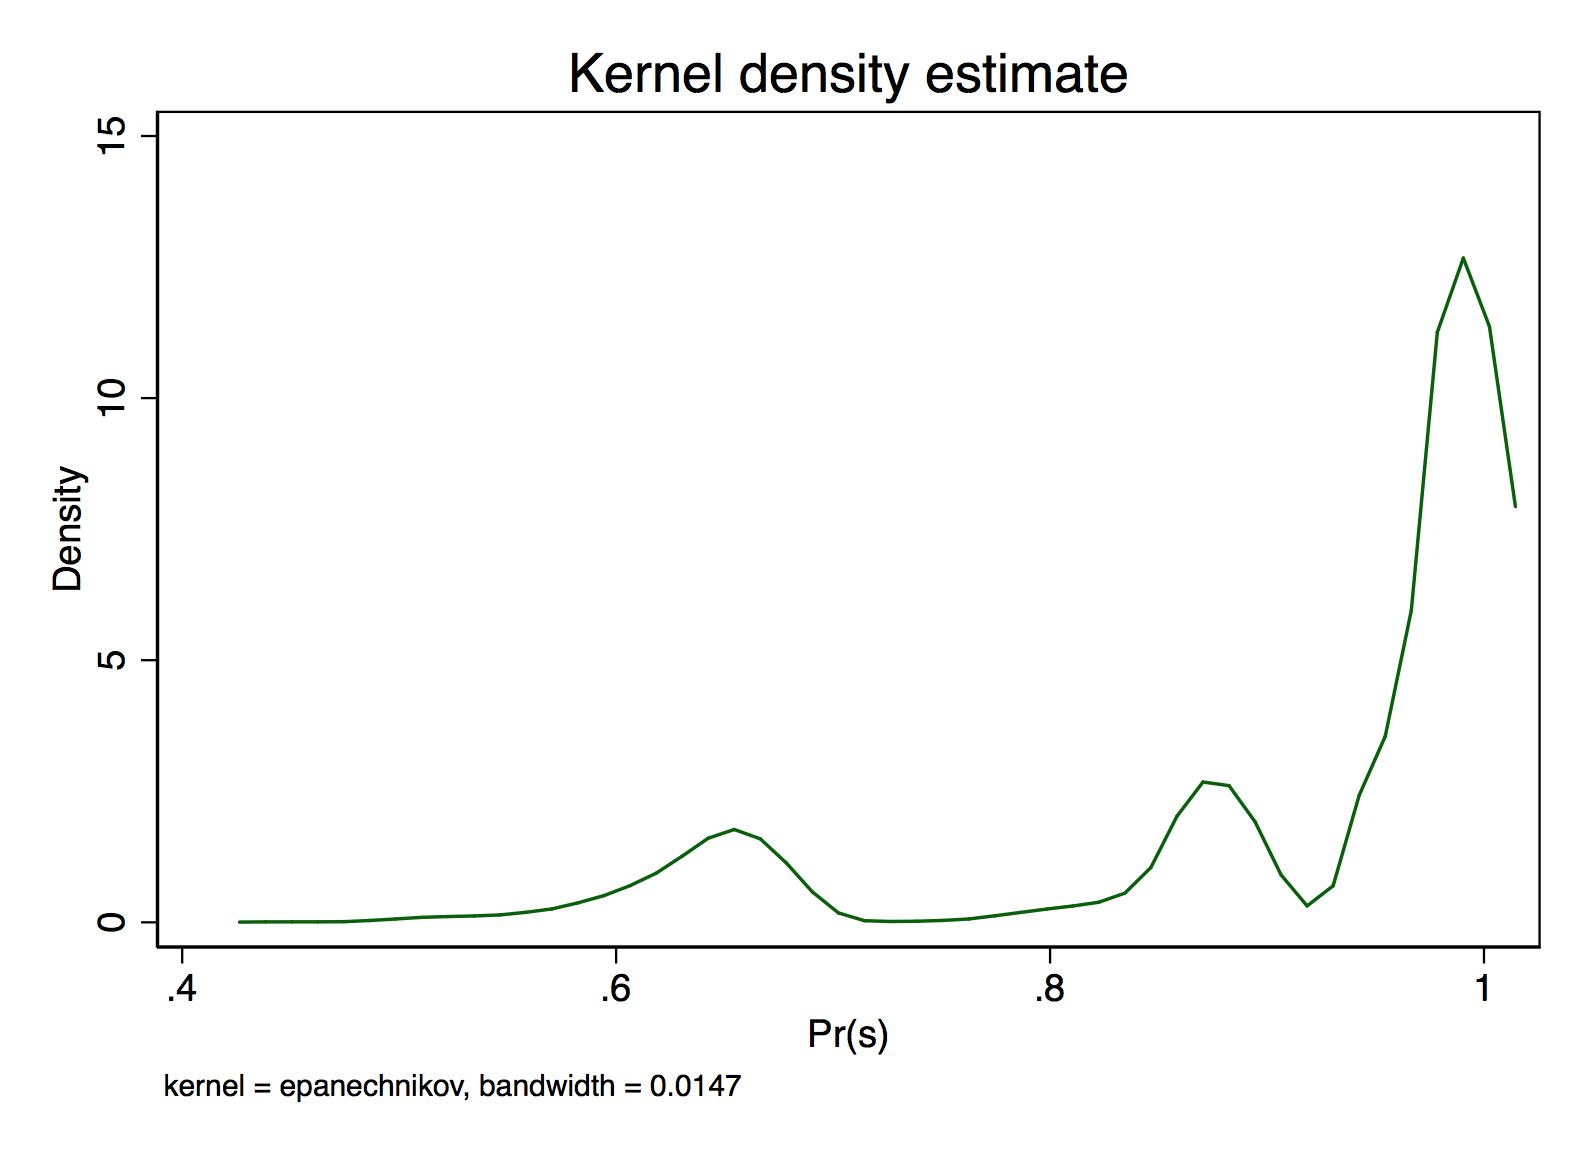
\includegraphics[totalheight=9cm]{hw3_q1_9a_stata.png}\\
\clearpage
\textbf{R output:}\\

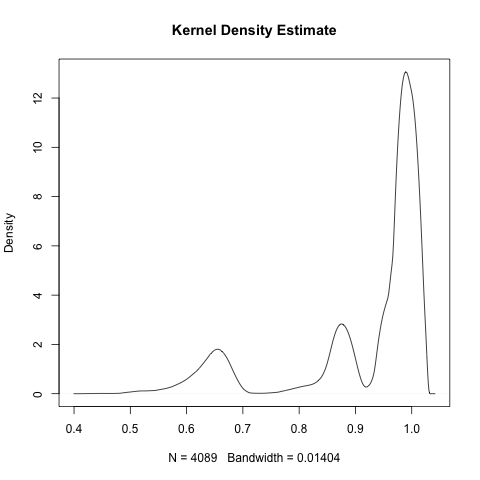
\includegraphics[totalheight=9cm]{hw3_q1_9c_r.png}\\





\newpage
\section{Semiparametric GMM with Missing Data}
\subsection{}
\subsubsection{}
Consider the following moment condition of a GMM estimatior:

\begin{align*}
  \E[m\mathbf{(y_i^*,t_i,x_i;\beta_0)}|t_i,x_i] = 0
\end{align*}

by the law of iterated expectations, the following conditions hold as well.

\begin{align*}
  \E[g\mathbf{(t_i,x_i)}\E[m\mathbf{(y_i^*,t_i,x_i;\beta_0)}|t_i,x_i] &= 0 \\
    \E[\E[g\mathbf{(t_i,x_i)}m\mathbf{(y_i^*,t_i,x_i;\beta_0)}|t_i,x_i]] &= 0 \\
      \E[g\mathbf{(t_i,x_i)}m\mathbf{(y_i^*,t_i,x_i;\beta_0)}|t_i,x_i] &= 0 , \ \forall g\mathbf{(t_i,x_i)}
\end{align*}

In order to find the function $g_0\mathbf{(t_i,x_i)}$ that minimizes asymptotic variance of the estimator, we write down the objective function and take first order conditions.


\begin{align*}
  \hat\beta = \arg \min_{\hat\beta} \left( \frac{1}{n} \qsum g\mathbf{(t_i,x_i)}m\mathbf{(y_i^*,t_i,x_i;\hat\beta)} \right)' W \left( \frac{1}{n} \qsum g\mathbf{(t_i,x_i)}m\mathbf{(y_i^*,t_i,x_i;\hat\beta)} \right)
\end{align*}

F.O.C.
\begin{align*}
  0 = \left( \frac{1}{n} \qsum \frac{\partial}{\partial\beta} g\mathbf{(t_i,x_i)}m\mathbf{(y_i^*,t_i,x_i;\hat\beta)} \right)' W \left( \frac{1}{n} \qsum \frac{\partial}{\partial\beta} g\mathbf{(t_i,x_i)}m\mathbf{(y_i^*,t_i,x_i;\hat\beta)} \right)
\end{align*}


Next we take a first order taylor expansion of the m function around $\beta_0$:

\begin{align*}
  0 &= \left( \frac{1}{n} \qsum \frac{\partial}{\partial\beta} g\mathbf{(t_i,x_i)}m\mathbf{(y_i^*,t_i,x_i;\beta_0)} \right)' W \left( \frac{1}{n} \qsum \frac{\partial}{\partial\beta} g\mathbf{(t_i,x_i)}m\mathbf{(y_i^*,t_i,x_i;\beta_0)} \right)\\
  & + \left( \frac{1}{n} \qsum \frac{\partial}{\partial\beta} g\mathbf{(t_i,x_i)}m\mathbf{(y_i^*,t_i,x_i;\beta_0)} \right)' W \left( \frac{1}{n} \qsum \frac{\partial}{\partial\beta} g\mathbf{(t_i,x_i)}m\mathbf{(y_i^*,t_i,x_i;\beta_0)} \right)(\hat\beta-\beta_0)
\end{align*}

and rearrange and multiply be $\sqrt{n}$ to give us the influence function

\begin{align*}
\sqrt{n} (\hat\beta - \beta_0) = \left(  \mathbf{\Omega_0'W\Omega_0} \right)^{-1} \Omega_0 W_0 \frac{1}{\sqrt{n}} \qsum \frac{\partial}{\partial\beta} g\mathbf{(t_i,x_i)}m\mathbf{(y_i^*,t_i,x_i;\beta_0)} + o_p(1)
\end{align*}

So by the CLT, assuming finite mean and variance of the estimator

\begin{align*}
\sqrt{n} (\hat\beta - \beta_0) \rightarrow_d N(0,V_0)
\end{align*}

where

\begin{align*}
  V_0 = \left(  \mathbf{\Omega_0'W\Omega_0} \right)^{-1} \mathbf{\Omega_0 W \Sigma_0 W \Omega_0} \left(  \mathbf{\Omega_0'W\Omega_0} \right)^{-1}
\end{align*}

and

\begin{align*}
  \Sigma_0 = \V[g\mathbf{(t_i,x_i)}m\mathbf{(y_i^*,t_i,x_i;\beta_0)}]
\end{align*}

Thus, the asymptotic variance is minimized when
\begin{align}
  \mathbf{W^* = \Sigma_0^{-1}}
\end{align}

and

\begin{align*}
g^*\mathbf{(t_i,x_i)} = \frac{\partial m_i}{\partial \beta} \V [ m\mathbf{(y_i^*,t_i,x_i;\beta_0)} |t_i,x_i]^{-1}
\end{align*}

which implies that $V_0^* = \left(  \Omega_0'\Sigma_0^{-1}  \Omega_0 \right)^{-1}$

Cool? Cool. Ok now we apply our findings to the model specified by the question.


\begin{align*}
\V [ m\mathbf{(y_i^*,t_i,x_i;\beta_0)} |t_i,x_i] =  F(t_i \theta_0 + x_i\gamma_0)(1 - F(t_i \theta_0 + x_i\gamma_0))
\end{align*}

and


\begin{align*}
\E [\frac{\partial m_i}{\partial \beta} |t_i,x_i] =  f(t_i\theta_0 + x_i*\gamma_0) [t_i,x_i']'
\end{align*}

which gives us our result

\begin{align*}
  g_0\mathbf{(t_i,x_i)} = \frac{f(t_i\theta_0 + x_i\gamma_0)}{F(t_i \theta_0 + x_i\gamma_0)(1 - F(t_i \theta_0 + x_i\gamma_0))} [t_i,x_i']'
\end{align*}

Now if the link function is the logistic cdf, then

$F(x) = \frac{1}{1+\exp(-x)}$ and $f(x) = \frac{-\exp(-x)}{(1+\exp(-x))^{2}} = -\exp(-x)F(x)^2$. So

\begin{align*}
 \frac{f(t_i\theta_0 + x_i\gamma_0)}{F(t_i \theta_0 + x_i\gamma_0)(1 - F(t_i \theta_0 + x_i\gamma_0))} [t_i,x_i']' &= \frac{-\exp(-x)F(x)^2}{(F(x))(1-F(x))} \\
 &= \frac{-\exp(-x)F(x)}{1-F(x)} \\
 &=1
\end{align*}

gives us $g_0\mathbf{(t_i,x_i)} = [t_i,x_i']'$

\subsection{}
\subsubsection{}
Using the previous result, the optimal moment condition is
\begin{align*}
\E[g\mathbf{(t_i,x_i)}m(y^*_i,t_i,x_i;\beta_0)] = 0
\end{align*}

As the outcome variable is missing at completely random, $s_i \bot (y^*_i,t_i,x_i;\beta_0)$

\begin{align*}
\E[g_0\mathbf{(t_i,x_i)}m(y^*_i,t_i,x_i;\beta_0)] &= 0\\
\E[g_0\mathbf{(t_i,x_i)}m(y^*_i,t_i,x_i;\beta_0)|s_i=1] &= 0
\end{align*}

Thus, the infesible estimator
\begin{align*}
  \hat\beta_{MCAR} = \arg \min_{\hat\beta_{MCAR}}  \left| \hat\E[g_0\mathbf{(t_i,x_i)}m(y^*_i,t_i,x_i;\hat\beta_{MCAR})|s_i=1]   \right|
\end{align*}
 is a consistent estimator of $\beta_0$, and we can construct the feasible estimator
 \begin{align*}
      \hat\beta_{MCAR,feasible} = \arg \min_{\hat\beta_{MCAR,feasible}} \left| \hat\E[\hat g\mathbf{(t_i,x_i)}m(y^*_i,t_i,x_i;\hat\beta_{MCAR})|s_i=1]   \right|
 \end{align*}


\subsubsection{}

\textbf{Stata output:}\\


\begin{tabular}{lcc}
\hline
&           $\hat \beta_{MCAR}$&     $CI_{95}$\\
\hline
dpisofirme  &   -.3163832&-.4476255,-.1851408\\
S\_age       &    -.244022&-.282266,-.2057781\\
S\_HHpeople  &     .023667&.0009192,.0464149\\
ls\_incomepc &    .0325661&.0073571,.057775\\
\end{tabular}

\vspace{1cm}
\textbf{R output:}\\

\begin{tabular}{lccc}
\hline
 & $\hat \beta_{MCAR}$  & $CI_{95}$ lower & $CI_{95}$ upper \\
  \hline
dpisofirme & -0.33 &  -0.52 & -0.17 \\
  S\_age & -0.23 &  -0.27 & -0.18 \\
  S\_HHpeople & 0.03 & -0.01 & 0.06 \\
  log\_inc & 0.02 &  -0.01 & 0.06 \\
   \hline
\end{tabular}

\subsection{}

\subsubsection{}
By previous result and Woodridge thm 14.4, the optimal instrument is derived from the variance
\begin{align*}
  \mathbf{\Omega_0(x_i)} &= \V[s_i m(t_i,x_i)|x_i,t_i]\\
  & = \E[s_i^2|x_i,t_i]F(t_i\theta+\mathbf{x_i'\gamma})(1-F(t_i\theta+\mathbf{x_i'\gamma})
\end{align*}

and

\begin{align*}
  \mathbf{M_0(x_i)} &=  \E[s_i^2|x_i,t_i]\E[m(t_i,\mathbf{x_i})]|\mathbf{x_i},t_i]
\end{align*}

Since $g_0(t_i,x_i) =  \mathbf{\Omega_0(x_i)^{-1}M_0(x_i)}$

\begin{align*}
  g_0\mathbf{(t_i,x_i)} = \frac{f(t_i\theta_0 + x_i\gamma_0)}{F(t_i \theta_0 + x_i\gamma_0)(1 - F(t_i \theta_0 + x_i\gamma_0))} [t_i,x_i']'
\end{align*}



\subsubsection{}


You can estimate $\beta_{MAR}$ through straight forward GMM, using the method described above. $\hat\beta_{MAR}$ and $\tilde\beta_{MAR}$ are asymptotically both asymptotically equivalent since we assume the conditional independence of the missing outcome indicator. Thus, the asymptotic equivalence is relative immediate from the moment condition listed in the problem using the law of iterated expectations.

That said, since the propensity score is unkown, additional variability is introduced through its estimation, thus it is safe to say that $\V^{Asy.} _{\hat\beta_{MAR}} \leq \V^{Asy.} _{\tilde\beta_{MAR}}$

\subsubsection{}
\textbf{Stata output:}\\

\begin{tabular}{lcc}
\hline
&           $\hat \beta_{MCAR}$ &     $CI_{95}$\\
\hline
S\_age       &   -.2446852 &-.2850008,-.2043697\\
S\_HHpeople  &    .0241638 &-.0019753,.050303\\
ls\_incomepc &    .0324512 &.0051728,.0597295\\
dpisofirme  &    -.315488 &-.4492407,-.1817353\\
\hline
\end{tabular}

\vspace{1cm}
\textbf{R output:}\\
\begin{tabular}{lccc}
  \hline
  & $\hat \beta_{MCAR}$  & $CI_{95}$ lower & $CI_{95}$ upper \\
  \hline
dpisofirme & -0.32  & -0.49 & -0.16  \\
  S\_age & -0.22 & -0.27 & -0.17 \\
  S\_HHpeople & 0.03  & -0.01 & 0.06 \\
  log\_inc & 0.02 &  -0.01 & 0.06 \\
   \hline
\end{tabular}

The estimates are consistent across software.

\subsubsection{}
\textbf{Stata output:}\\

\begin{tabular}{lcc}
\hline
&           $\hat \beta_{MAR}$ &     $CI_{95}$\\
\hline
S\_age       &   -.2446852&-.2822807,-.2070897\\
S\_HHpeople  &    .0241638&.0000545,.0482732\\
ls\_incomepc &    .0324512&.0068349,.0580674\\
dpisofirme  &    -.315488&-.4485709,-.1824051\\
\hline
\end{tabular}

\vspace{1cm}
\textbf{R output:}\\
\begin{tabular}{lccc}
  \hline
  & $\hat \beta_{MAR}$  & $CI_{95}$ lower & $CI_{95}$ upper \\
  \hline
  dpisofirme & -0.32  & -0.49 & -0.16 \\
    S\_age & -0.22 & -0.27 & -0.17 \\
    S\_HHpeople & 0.03  & -0.01 & 0.06 \\
    log\_inc & 0.02  & -0.01 & 0.06 \\
\hline
\end{tabular}

The point estimates are consistent across software. The variances differ slightly. I have not found what is leading to the difference. The results do not change a lot since the propensity scores of the sample are significantly far from 0.

\newpage
\section{When Bootstrap Fails}
\subsection{}
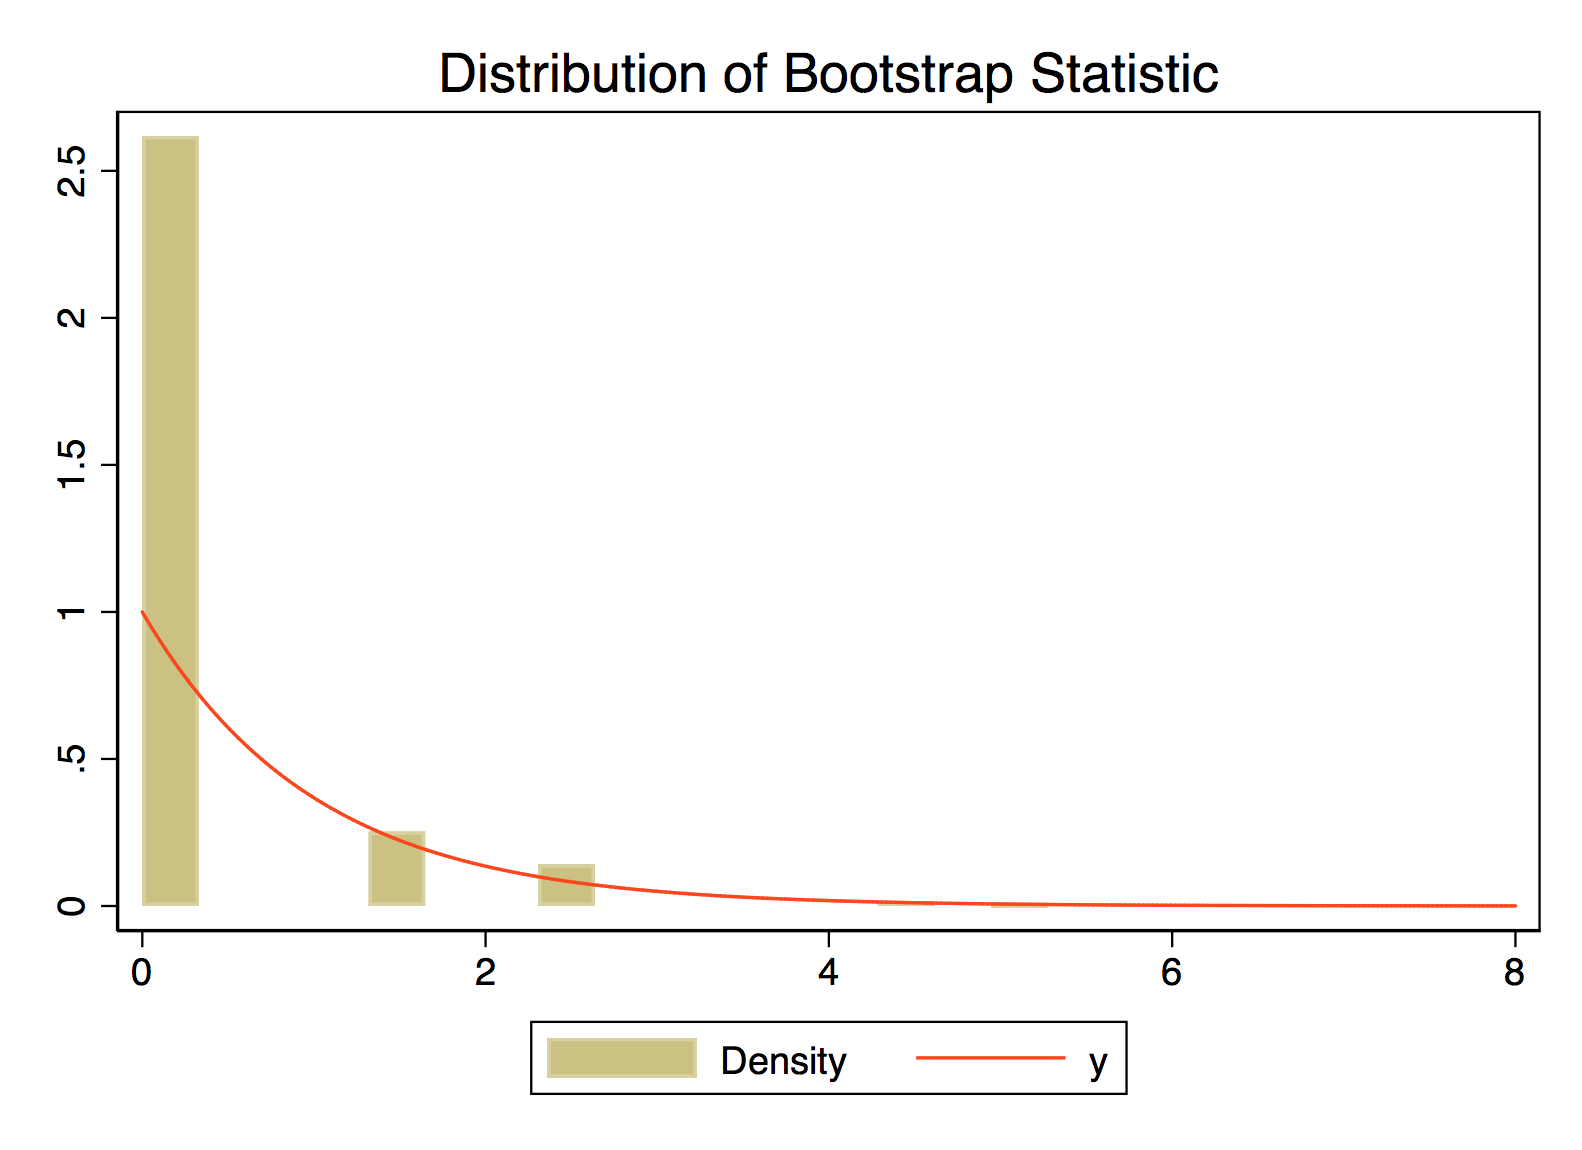
\includegraphics[totalheight=6cm]{hw3_Q3_1_stata.png}
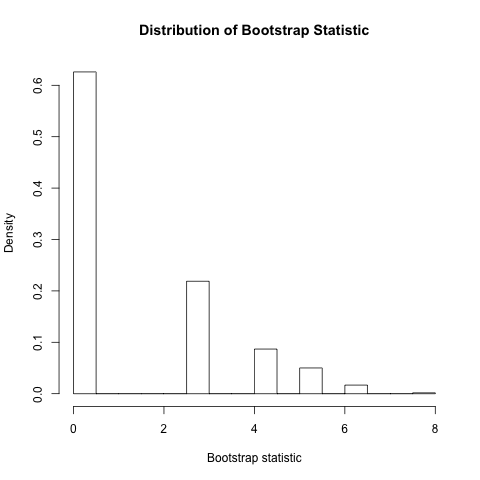
\includegraphics[totalheight=6cm]{hw3_q3_2_r.png}\\

No, it does not coincide with the theoretical Exponential(1) distribution. The plots appear similar.
\subsection{}
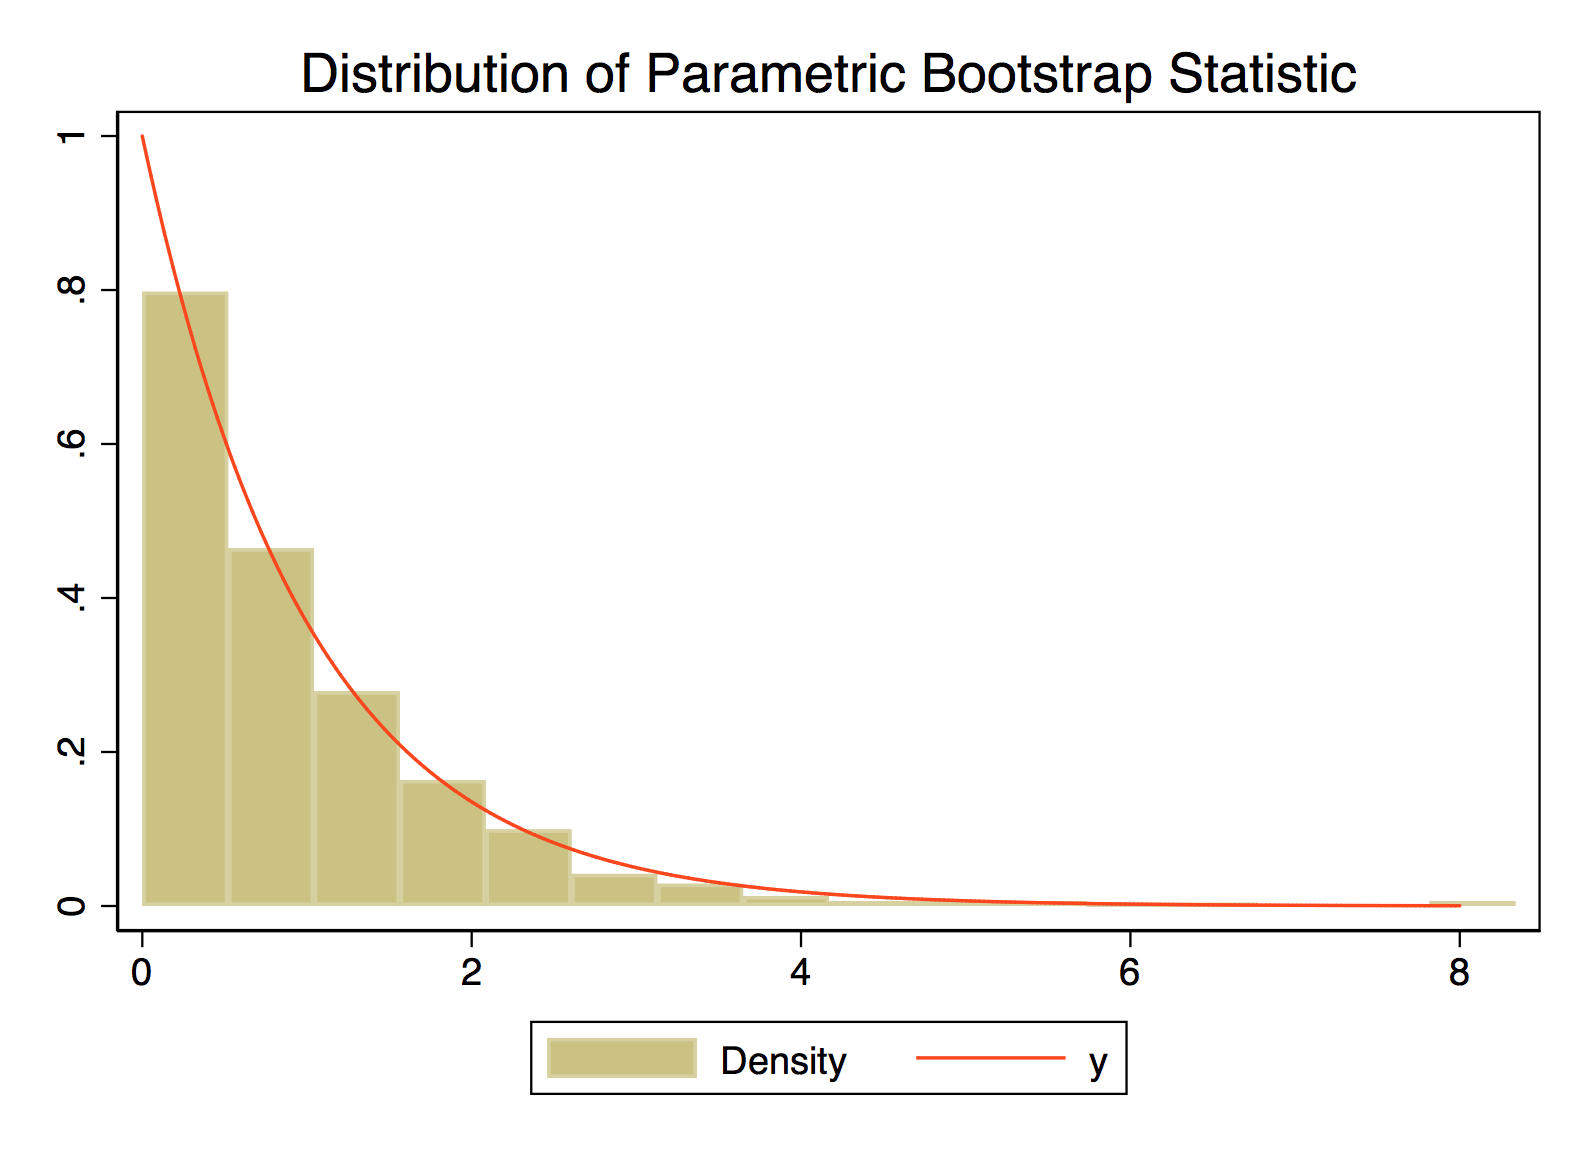
\includegraphics[totalheight=6cm]{hw3_Q3_2_stata.png}
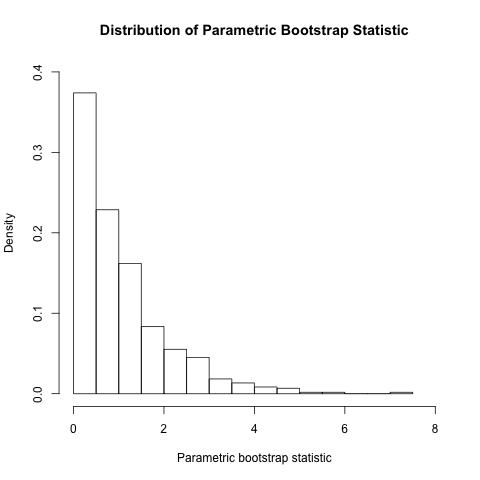
\includegraphics[totalheight=6cm]{hw3_q3_3_r.png}\\

Yes, it does coincide with the theoretical Exponential(1) distribution. The plots appear similar.
\subsection{}

The intuitive reason behind why the nonparametic bootsstrap fails is that by this method $ \E[\max_i x^*_i] = \frac{2}{n}\qsum x_i \neq \max_i x_i$.

While in the case of the parametric it works out, as $ \E[\max_i x^*_i] = \max_i x_i$ by construction



\newpage
\section{Code Appendix}
\tiny
\subsection*{Stata}
\lstinputlisting{hw3.do}
\subsection*{R}
\lstinputlisting{hw3_q1.R}
\lstinputlisting{hw3_q2.R}
\lstinputlisting{hw3_q3.R}
\end{document}
